\section*{Eliminar el offset de los amplificadores operacionales}

El offset en aplicaciones de instrumentación electrónica que requieran de precisión o un control exacto o de bajo error en la salida dependen en gran medida del nivel de offset calibrado en cada elemento de control, siendo así necesario eliminar este elemento de disparidad al medir la salida de un operacional, aplicando para este paso fundamental el agregado de potenciómetros de 10K $\Omega$ para cada operacional del $LM741$ en sus pines 1 y 5 respectivamente con una referencia positiva de voltaje.

% TODO: \usepackage{graphicx} required
\begin{figure}[h]
	\centering
	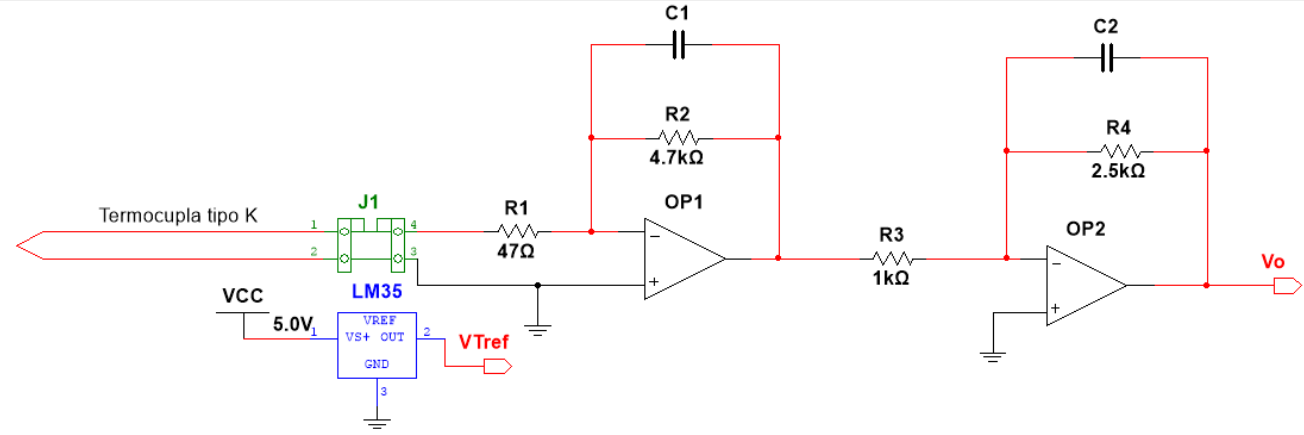
\includegraphics[width=0.8\linewidth]{media/amplificador-voltaje}
	\caption{Circuito amplificador de voltaje}
	\label{fig:amplificador-voltaje}
\end{figure}

En la figura \ref{fig:amplificador-voltaje} se muestra el circuito de amplificación destacando dentro de este mismo los operacionales y sus respectivas salida, siendo así que para obtener un valor nulo de offset para cada uno es necesario obtener un voltaje equivalente a 0 ó muy cercano en cada salida, obteniendo así la tabla \ref{tab:sup-offset}

\begin{table}[h]
	\centering
	\begin{tabular}{|ll|}
		\hline
		\multicolumn{2}{|c|}{\textbf{Offset Amp. Op}}                 \\ \hline
		\multicolumn{1}{|l|}{\textbf{VoffsetOp1 {[}V{]}}}      & 8.24 \\ \hline
		\multicolumn{1}{|l|}{\textbf{VoffsetOp2 {[}V{]}}}      & 9.58 \\ \hline
		\multicolumn{1}{|l|}{\textbf{VoffsetNullOp1 {[}mV{]}}} & 680  \\ \hline
		\multicolumn{1}{|l|}{\textbf{VoffsetNullOp2 {[}mV{]}}} & 798  \\ \hline
	\end{tabular}
	\caption{Medición y supresión del offset}
	\label{tab:sup-offset}
\end{table}